% =============================================================================
% Dengue forecasting benchmark, eight Brazilian state capitals (2010 to 2024)
%
% Tabelas e figuras sao geradas por scripts/build_paper_assets.py e incluidas
% daqui. Nao editar paper/tables/*.tex a mao: rode o script.
% Todo numero citado no corpo do texto esta em paper/verified_numbers.json.
%
% Compilar:  latexmk -pdf manuscript.tex     (ou make -C paper)
% =============================================================================
\documentclass[11pt]{article}

\usepackage[margin=1in]{geometry}
\usepackage[T1]{fontenc}
\usepackage[utf8]{inputenc}
\usepackage{lmodern}
\usepackage{setspace}
\usepackage{booktabs}
\usepackage{multirow}
\usepackage{graphicx}
\usepackage{xurl}
\usepackage{lineno}
\usepackage[round,authoryear]{natbib}
\usepackage{xcolor}
\usepackage{caption}

\captionsetup{font=small,labelfont=bf}
\graphicspath{{figures/}}

% marcador de dado ainda nao disponivel, visivel na compilacao
\newcommand{\missing}[1]{\textcolor{red}{\textbf{[MISSING: #1]}}}

\title{Zero-Shot Foundation Models Versus Purpose-Trained Models for Dengue
Forecasting in Eight Brazilian State Capitals (2010 to 2024):\\
A Rolling-Origin Benchmark}

\author{Fabiano Barcellos-Filho\thanks{Corresponding author:
\texttt{fabiano.nb@gmail.com}} \and Jos\'e Trajano \and Wilson Falco}

\date{}

\setstretch{1.5}
\linenumbers

\begin{document}

\maketitle

% =============================================================================
\begin{abstract}
\noindent\textbf{Background.} Dengue imposes a recurrent and heavy burden on the
Brazilian health system, and municipal forecasts are used to plan vector control,
procurement and hospital capacity. Operational forecasting tools rely on models that
must be trained and periodically retrained for each city, which limits how widely they
can be deployed. Whether a pre-trained time-series foundation model can substitute for
that per-city pipeline has not been tested on Brazilian dengue data.

\noindent\textbf{Methods.} We benchmarked seven forecasting models on monthly notified
dengue counts from InfoDengue for eight Brazilian state capitals covering January 2010
to December 2024 (180 monthly observations per city). Six models were trained per city
(SARIMAX, Ridge regression, LightGBM, XGBoost, CatBoost and Random Forest, the last five
using recursive multi-step forecasting with 24 autoregressive lags), and one, TimesFM
2.5, was applied zero-shot with no city-specific training. Evaluation used rolling-origin
cross-validation with an expanding window (minimum training window 48 months, forecast
horizon 12 months, step 1 month), producing 121 folds and 1{,}452 pooled predictions per
model per city and 81{,}312 predictions overall. The pre-specified primary metric was
sMAPE; MAE and RMSE were reported alongside it. Uncertainty was quantified by bootstrap
resampling of the pooled predictions (2{,}000 replicates, percentile method). Reporting
follows TRIPOD+AI.

\noindent\textbf{Results.} TimesFM achieved the lowest sMAPE in seven of eight cities
(mean across cities 75.3\%, range 56.0\% to 97.1\%) against 85.6\% for CatBoost, the best
purpose-trained model, 105.2\% for Ridge, 105.5\% for SARIMAX and 114.6\% for LightGBM. By
MAE, TimesFM ranked first in all eight cities. The largest margin was in Rio de Janeiro
(sMAPE 96.8\%, 95\% CI 94.0 to 99.4, versus 119.7\%, 116.7 to 122.6, for XGBoost). In
S\~ao Paulo the two leading models were indistinguishable (78.0\%, 75.2 to 80.8, versus
78.7\%, 75.7 to 81.7, for CatBoost). The three metrics selected the same model in only
four of eight cities: in Belo Horizonte each metric named a different winner, XGBoost on
sMAPE, TimesFM on MAE and Ridge on RMSE. All models substantially underestimated the 2024
epidemic peaks.

\noindent\textbf{Conclusion.} A zero-shot foundation model matched or exceeded
purpose-trained models for 12-month-ahead dengue forecasting across heterogeneous
Brazilian capitals without any local training, which lowers the cost of extending
forecasting to municipalities that lack modelling capacity. Absolute error remained
large in every city and no model anticipated the 2024 epidemic, so these forecasts are
suited to planning baselines rather than outbreak triggers.

\vspace{0.8em}
\noindent\textbf{Keywords:} dengue; forecasting; foundation model; time series;
machine learning; Brazil; epidemiological surveillance
\end{abstract}

% =============================================================================
\section{Introduction}

Dengue is the most widespread arboviral disease globally, and tropical Latin America
carries one of the heaviest burdens \citep{Leung2023}. Brazil reported the largest
epidemic in its recorded history in 2024, with outbreaks across all five macroregions
\citep{GurgelGoncalves2024}. The consequences reach beyond case counts: direct treatment
costs, lost productivity and crowding of primary care and emergency services concentrate
in exactly the regions with the least surge capacity \citep{Siqueira2022}.

Forecasting has an established place in this response. Reliable anticipation of case
volume allows health authorities to preposition supplies, time vector control and plan
hospital capacity before a peak \citep{Roster2022}. Brazil is unusually well equipped for
this: InfoDengue, operated jointly by Fiocruz and FGV, integrates notification records
from SINAN and publishes near-real-time municipal surveillance data
\citep{Codeco2018infodengue}. What the country lacks is an integrated forecasting layer
able to serve the diversity of local epidemic dynamics.

Two gaps limit the existing evidence. First, a systematic review of dengue forecasting
found that studies rarely report calibration, seldom use comparable validation designs,
and derive performance predominantly from internal validation, which makes quantitative
synthesis across methods impossible \citep{Leung2023}. Second, and more consequential for
deployment, the models that perform best are trained city by city. In S\~ao Paulo,
generalised additive models outperformed ARIMA and neural networks; across multiple
Brazilian cities, the best model differed by city \citep{Chen2025rj,Fang2024}. A national
surveillance programme covering thousands of municipalities cannot maintain a bespoke
pipeline for each one.

Time-series foundation models offer a different arrangement. Pre-trained on large and
heterogeneous temporal corpora, they generate forecasts without any task-specific
training \citep{Das2024timesfm,Ansari2024chronos,Woo2024moirai}. If such a model performs
comparably to purpose-trained alternatives on dengue series, the marginal cost of
extending forecasting to an additional municipality falls to the cost of running
inference. Whether that transfers to dengue counts, which are volatile, strongly seasonal
and punctuated by epidemics an order of magnitude above baseline, has not been tested.

This study therefore aimed to: (i) describe the evolution of dengue incidence across
eight Brazilian state capitals over 15 years; (ii) benchmark a zero-shot foundation model
against six purpose-trained forecasting models under a single standardised
rolling-origin validation design; and (iii) characterise periods of critical
epidemiological burden using scan statistics, in order to situate forecast error against
the epidemic phases that matter operationally.

% =============================================================================
\section{Methods}

Reporting follows the TRIPOD+AI statement for the development and evaluation of
prediction models using regression or machine learning methods
\citep{Collins2024tripod}. All data are publicly available aggregate surveillance records
with no individual-level information, so ethics committee review was not required.
Analysis code, processed data and every result file underlying the tables and figures are
openly available at \url{https://github.com/fabianofilho/dengue-time-series}.

\subsection{Study setting and data source}

Eight Brazilian state capitals were studied: S\~ao Paulo (SP), Rio de Janeiro (RJ), Belo
Horizonte (MG), Bras\'ilia (DF), Fortaleza (CE), Recife (PE), Manaus (AM) and Salvador
(BA). Together they span the Southeast, Central-West, Northeast and North macroregions
and cover a wide range of climatic, demographic and transmission profiles.

Notification data were obtained through the InfoDengue public API
(\url{https://info.dengue.mat.br/}), which aggregates mandatory notifications from SINAN
\citep{Codeco2018infodengue}. Weekly counts for epidemiological week 1 of 2010 through
week 52 of 2024 were aggregated to calendar months using the month-start convention,
yielding 180 monthly observations per city and 1{,}440 city-months in total.

\subsection{Outcome and predictors}

The outcome was the monthly count of notified dengue cases per city, modelled on its
original scale with no transformation. Forecasts below zero were clipped to zero.

No exogenous covariates were used. This is a deliberate constraint: it holds the feature
set identical across all seven models, so that differences in accuracy are attributable to
the forecasting architecture rather than to unequal access to information. The six
purpose-trained models used 24 autoregressive lags of the monthly count, a two-year
lookback chosen to span the dominant inter-annual dengue cycle in Brazil. The
consequences of excluding climate covariates are addressed in the limitations.

\subsection{Models}

\textbf{SARIMAX} served as the parametric statistical baseline, with non-seasonal order
$(1,1,1)$ and seasonal order $(1,1,0)_{12}$, estimated by maximum likelihood in
\texttt{statsmodels}. Orders were fixed across cities and folds rather than selected per
fold, which reflects realistic deployment but may understate its optimised performance.

\textbf{Ridge regression} provided a linear autoregressive baseline on the same 24 lags,
with the default L2 penalty. Unlike the tree ensembles, Ridge is not scale-invariant, and
the lags were standardised before fitting. This is not a cosmetic choice. Without
standardisation the penalty is negligible relative to counts in the thousands, and in the
earliest folds, where the number of training rows approaches the number of lags, the fit
becomes near-singular; recursive 12-step prediction then amplifies the result. In
Salvador a single fold, the one with 49 months of training, produced a forecast of
$8.7 \times 10^{14}$ cases and by itself dominated that city's pooled MAE and RMSE. After
standardisation no fold diverged in any city. We report this because the failure is
nearly silent under sMAPE, which is bounded and therefore absorbs a divergence of any
magnitude: the unscaled Salvador run returned a plausible-looking sMAPE of 96.3\% while
its MAE was $6.7 \times 10^{11}$.

\textbf{LightGBM, XGBoost, CatBoost and Random Forest}
\citep{Ke2017lightgbm,Chen2016xgboost,Prokhorenkova2018catboost,Breiman2001} were wrapped
in the recursive multi-step forecaster of \texttt{skforecast}
(\texttt{ForecasterRecursive}) with 24 lags. Each was refitted independently at every
fold on the data available at that point. Library defaults were used with a fixed random
seed; no hyperparameter search was performed, for the same reason the SARIMAX orders were
fixed.

\textbf{TimesFM 2.5} is a 200-million-parameter decoder-only transformer pre-trained by
Google DeepMind on a large multi-domain corpus of time series \citep{Das2024timesfm}. It
was loaded from the HuggingFace Hub (checkpoint
\texttt{google/timesfm-2.5-200m-pytorch}), with maximum context 512, maximum horizon 24,
input normalisation on and a positivity constraint. It was used strictly zero-shot: no
fine-tuning, no city-specific adaptation and no refitting at any fold. It therefore
receives strictly less information than its competitors, which see the city's own
training window at every fold.

One model specified in the study protocol was not evaluated and is reported here for
completeness. Prophet \citep{Taylor2018prophet} failed to run in seven of the eight
cities because of an unresolved dependency, and partial results from a single city are
not interpretable as a benchmark. It does not appear in the results and is not discussed
as though it had been tested.

\subsection{Evaluation design}

We used rolling-origin cross-validation with an expanding training window
\citep{Tashman2000,Hewamalage2023}. At each fold the model is fitted only on observations
preceding the forecast origin and predicts the following 12 months, so no information
from the evaluation period reaches the model \citep{Kapoor2023}. The minimum training
window was 48 months, chosen so that every supervised model sees at least two complete
annual cycles before its first forecast; the origin then advances one month at a time.

For a series of length $T = 180$ with minimum training size $m = 48$ and horizon
$h = 12$, this yields $T - m - h + 1 = 121$ folds per city, $121 \times 12 = 1{,}452$
predictions per model per city, and $1{,}452 \times 7 \times 8 = 81{,}312$ predictions in
total.

This is temporal out-of-sample evaluation within a single data source, which is internal
validation under the TRIPOD+AI nomenclature. It is not external validation: no
independent cohort, surveillance system or country was used. The eight cities are eight
separate internal validations, not a geographic external validation, because each
purpose-trained model is fitted on the same city it is evaluated in.

\subsection{Performance metrics and uncertainty}

The primary metric, declared before analysis, was sMAPE, computed on predictions pooled
across all folds within a city:
\[
\mathrm{sMAPE} = \frac{100}{n}\sum_{t=1}^{n}
\frac{|y_t - \hat{y}_t|}{(|y_t| + |\hat{y}_t|)/2}.
\]
sMAPE is bounded and treats over- and under-forecasting symmetrically, which suits series
that spend most months near a low baseline and occasionally spike
\citep{Hewamalage2023}. MAE and RMSE were reported alongside it on the original case
scale. The three are reported together because they reward different behaviour: sMAPE
rewards accuracy in inter-epidemic troughs, RMSE rewards accuracy at peaks, and reporting
only one would conceal the disagreement quantified in Table~\ref{tab:metric-disagreement}.

Uncertainty was quantified by resampling the 1{,}452 paired predictions with replacement
(2{,}000 replicates, percentile method) to obtain 95\% intervals for sMAPE. Predictions
from the same rolling-origin fold, and from adjacent origins, are not independent;
these intervals therefore understate the true uncertainty and are interpreted throughout
as a lower bound on the spread rather than as a formal test. No hypothesis test of
model superiority was performed, and none is claimed.

\subsection{Cluster analysis}

Temporal and space-time clusters of dengue incidence were to be estimated with SaTScan
version 10.1 under a discrete Poisson model, using city-month population as the expected
count, with a maximum temporal window of 50\% of the study period and significance
assessed by 999 Monte Carlo replications at $p < 0.05$. Three scans were planned: a
purely temporal high-rate scan per city, a space-time scan across all eight cities, and a
purely temporal low-rate scan per city to characterise inter-epidemic troughs. Population
denominators were to come from IBGE intercensal estimates (2010 to 2022) and projections
(2023 to 2024), with city centroids from the IBGE Malha Municipal.

\missing{The SaTScan analysis has not been run. No cluster output, population denominator
file or centroid file exists in the project repository. Every cluster result in
Section~\ref{sec:clusters} is a placeholder. Either the analysis is executed and the
results inserted, or this objective and the corresponding aim in the Introduction are
removed before submission.}

\subsection{Software}

Python 3.12 with pandas, scikit-learn 1.3, skforecast, statsmodels 0.14, LightGBM,
XGBoost, CatBoost and timesfm. The full pipeline, from data acquisition through
backtesting to the generation of every table and figure in this manuscript, is
reproducible from the repository by running \texttt{scripts/build\_paper\_assets.py}.

% =============================================================================
\section{Results}

\subsection{Descriptive characteristics}

Table~\ref{tab:descriptive} summarises the eight series and Figure~\ref{fig:series} shows
them. The cities differ by more than an order of magnitude in burden: S\~ao Paulo
accumulated 1{,}711{,}689 notified cases over the period against 116{,}817 in Salvador.
They also differ in volatility. The coefficient of variation ranges from 108\% in
Salvador to 431\% in S\~ao Paulo, where the median month recorded 1{,}198 cases and the
peak month 331{,}402, a ratio of about 277 to 1. Manaus shows the same pattern at a smaller
scale (median 264, maximum 21{,}605). This concentration of the case burden into a
handful of months is the central difficulty for every model evaluated here, and it is
what separates the metrics in Section~\ref{sec:disagreement}.

% gerado por scripts/build_paper_assets.py -- nao editar a mao
\begin{table}[htbp]
\centering
\footnotesize
\setlength{\tabcolsep}{4pt}
\caption{Notified dengue burden in eight Brazilian state capitals, January 2010 to
December 2024: monthly case counts and population-standardised incidence.}
\label{tab:descriptive}
\begin{tabular}{llrrrrrrrr}
\toprule
 & & Pop. 2022 & \multicolumn{4}{c}{Monthly cases}
 & \multicolumn{3}{c}{Incidence per 100{,}000} \\
\cmidrule(lr){4-7} \cmidrule(lr){8-10}
City & Region & (millions) & Total & Median & Max & CV (\%)
 & Annual & Median & Max \\
\midrule
Belo Horizonte (MG) & Southeast & 2.32 & 1,081,180 & 948 & 113,951 & 262 & 3,124 & 41 & 4,938 \\
Brasilia (DF) & Central-West & 2.82 & 720,807 & 1,146 & 102,593 & 283 & 1,740 & 43 & 3,597 \\
Fortaleza (CE) & Northeast & 2.43 & 381,475 & 962 & 21,568 & 142 & 1,054 & 39 & 881 \\
Sao Paulo (SP) & Southeast & 11.45 & 1,702,694 & 1,192 & 342,838 & 432 & 1,002 & 10 & 2,986 \\
Recife (PE) & Northeast & 1.49 & 184,961 & 488 & 7,667 & 132 & 824 & 32 & 506 \\
Rio de Janeiro (RJ) & Southeast & 6.21 & 637,074 & 658 & 55,481 & 241 & 685 & 10 & 880 \\
Manaus (AM) & North & 2.06 & 132,030 & 274 & 19,556 & 285 & 472 & 14 & 1,078 \\
Salvador (BA) & Northeast & 2.42 & 116,190 & 344 & 4,088 & 106 & 312 & 13 & 171 \\
\bottomrule
\end{tabular}

\vspace{0.5em}
\begin{minipage}{\textwidth}
\footnotesize
Each city contributed 180 monthly observations. CV: coefficient of variation of the
monthly case count (standard deviation divided by the mean, as a percentage). Incidence
columns are notified cases per 100{,}000 inhabitants; Annual is the mean monthly
incidence multiplied by twelve, Median and Max are monthly values. Rows are sorted by
mean annual incidence, which reorders the table relative to absolute counts. Population
denominators are interpolated monthly from an annual series anchored on the 2010 and 2022
Censuses (see Methods). Case source: InfoDengue (Fiocruz/FGV); population source: IBGE.
\end{minipage}
\end{table}


\begin{figure}[htbp]
\centering
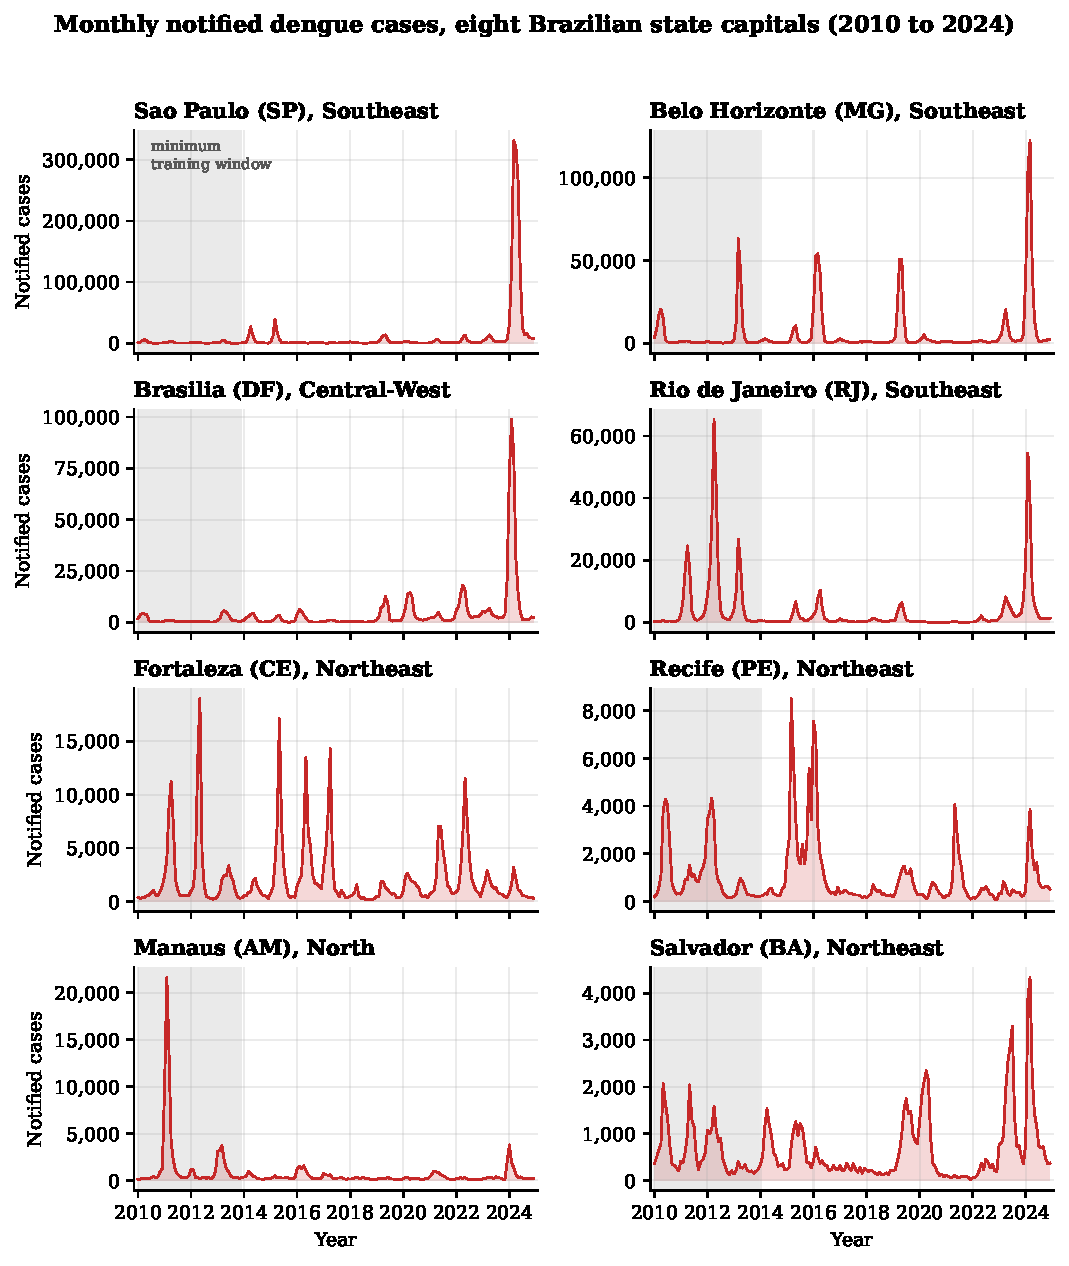
\includegraphics[width=\textwidth]{fig1_series.pdf}
\caption{Monthly notified dengue cases in eight Brazilian state capitals, January 2010 to
December 2024. Panels are ordered by cumulative case count and each has its own vertical
scale. The shaded band marks the 48-month minimum training window, before which no
forecast is evaluated. The 2024 epidemic is visible in all eight series.}
\label{fig:series}
\end{figure}

\subsection{Forecasting accuracy}

Table~\ref{tab:smape} reports sMAPE with bootstrap intervals and
Figure~\ref{fig:heatmap} displays the same values as a heatmap. TimesFM achieved the
lowest sMAPE in seven of eight cities, with a mean across cities of 75.3\% (range 56.0\%
in Manaus to 97.1\% in Belo Horizonte). The best purpose-trained model on the same
summary was CatBoost at 85.6\%, followed by XGBoost at 85.9\%, Random Forest at 89.3\%,
Ridge at 105.2\%, SARIMAX at 105.5\% and LightGBM at 114.6\%.

The margin varies sharply by city and the intervals matter for reading it. In Rio de
Janeiro the separation is wide and the intervals do not overlap: TimesFM 96.8\% (95\% CI
94.0 to 99.4) against 119.7\% (116.7 to 122.6) for XGBoost, the best supervised model
there. Manaus, Fortaleza and Recife show the same pattern of non-overlap. In S\~ao Paulo
the intervals overlap almost entirely, at 78.0\% (75.2 to 80.8) for TimesFM against
78.7\% (75.7 to 81.7) for CatBoost; the 0.7 percentage point gap there is not evidence of
an advantage and is not treated as one. Belo Horizonte is the one city where a supervised
model leads on the primary metric, with XGBoost at 88.7\% (85.3 to 92.0) against 97.1\%
(94.0 to 100.2) for TimesFM.

% gerado por scripts/build_paper_assets.py -- nao editar a mao
\begin{table}[htbp]
\centering
\footnotesize
\setlength{\tabcolsep}{2.5pt}
\caption{Forecasting accuracy by model and city: sMAPE (\%) with 95\% bootstrap
percentile confidence intervals. Rolling-origin cross-validation, 12-month horizon,
1{,}452 pooled predictions per model per city.}
\label{tab:smape}
\begin{tabular}{lccccccc}
\toprule
City & TimesFM & CatBoost & XGBoost & Random Forest & SARIMAX & Ridge & LightGBM \\
\midrule
Sao Paulo & \textbf{78.0} & 78.7 & 84.8 & 87.3 & 87.1 & 111.5 & 119.8 \\
 & \tiny(75.2, 80.8) & \tiny(75.7, 81.7) & \tiny(81.7, 87.8) & \tiny(84.4, 90.4) & \tiny(83.9, 90.2) & \tiny(108.4, 114.6) & \tiny(117.0, 122.7) \\[2pt]
Rio de Janeiro & \textbf{96.8} & 126.4 & 119.7 & 133.3 & 135.6 & 132.8 & 154.7 \\
 & \tiny(94.0, 99.4) & \tiny(123.6, 129.1) & \tiny(116.7, 122.6) & \tiny(130.5, 136.1) & \tiny(132.2, 138.8) & \tiny(129.7, 135.9) & \tiny(152.0, 157.4) \\[2pt]
Belo Horizonte & 97.1 & 95.2 & \textbf{88.7} & 90.2 & 134.0 & 133.0 & 151.4 \\
 & \tiny(94.0, 100.2) & \tiny(92.3, 98.3) & \tiny(85.3, 92.0) & \tiny(87.0, 93.6) & \tiny(130.6, 137.4) & \tiny(129.9, 136.0) & \tiny(148.7, 154.1) \\[2pt]
Brasilia & \textbf{74.3} & 76.6 & 83.7 & 82.4 & 103.2 & 114.4 & 100.5 \\
 & \tiny(71.6, 76.9) & \tiny(74.3, 79.1) & \tiny(81.2, 86.4) & \tiny(79.8, 85.1) & \tiny(99.9, 106.5) & \tiny(111.2, 117.7) & \tiny(97.7, 103.3) \\[2pt]
Fortaleza & \textbf{64.2} & 77.5 & 89.4 & 98.4 & 87.6 & 89.2 & 102.1 \\
 & \tiny(62.2, 66.2) & \tiny(75.0, 80.2) & \tiny(86.6, 92.1) & \tiny(95.7, 101.1) & \tiny(84.5, 90.7) & \tiny(86.3, 92.1) & \tiny(99.0, 105.0) \\[2pt]
Recife & \textbf{67.3} & 83.3 & 83.3 & 81.2 & 105.6 & 105.4 & 111.2 \\
 & \tiny(64.9, 69.6) & \tiny(80.6, 86.0) & \tiny(80.4, 86.4) & \tiny(78.5, 84.0) & \tiny(102.4, 108.8) & \tiny(102.4, 108.4) & \tiny(108.4, 113.9) \\[2pt]
Manaus & \textbf{56.0} & 70.9 & 65.5 & 67.9 & 99.7 & 62.5 & 94.8 \\
 & \tiny(53.9, 58.2) & \tiny(69.0, 72.8) & \tiny(63.5, 67.5) & \tiny(66.0, 69.7) & \tiny(96.3, 103.1) & \tiny(60.4, 64.6) & \tiny(92.4, 97.3) \\[2pt]
Salvador & \textbf{68.9} & 76.0 & 72.1 & 73.7 & 91.0 & 92.4 & 82.2 \\
 & \tiny(66.5, 71.2) & \tiny(73.8, 78.4) & \tiny(69.4, 74.7) & \tiny(71.1, 76.2) & \tiny(87.6, 94.2) & \tiny(89.5, 95.3) & \tiny(79.8, 84.4) \\[2pt]
\midrule
Mean across cities & \textbf{75.3} & 85.6 & 85.9 & 89.3 & 105.5 & 105.2 & 114.6 \\
Cities ranked first & \textbf{7/8} & 0/8 & 1/8 & 0/8 & 0/8 & 0/8 & 0/8 \\
\bottomrule
\end{tabular}

\vspace{0.5em}
\begin{minipage}{\textwidth}
\footnotesize
Bold indicates the lowest sMAPE in each row. Confidence intervals were obtained by
resampling the 1{,}452 paired predictions with replacement (2000 replicates,
percentile method). Because predictions from the same rolling-origin fold are not
independent, these intervals understate the true uncertainty and should be read as a
lower bound on the spread. TimesFM was applied zero-shot, with no city-specific
training.
\end{minipage}
\end{table}


\begin{figure}[htbp]
\centering
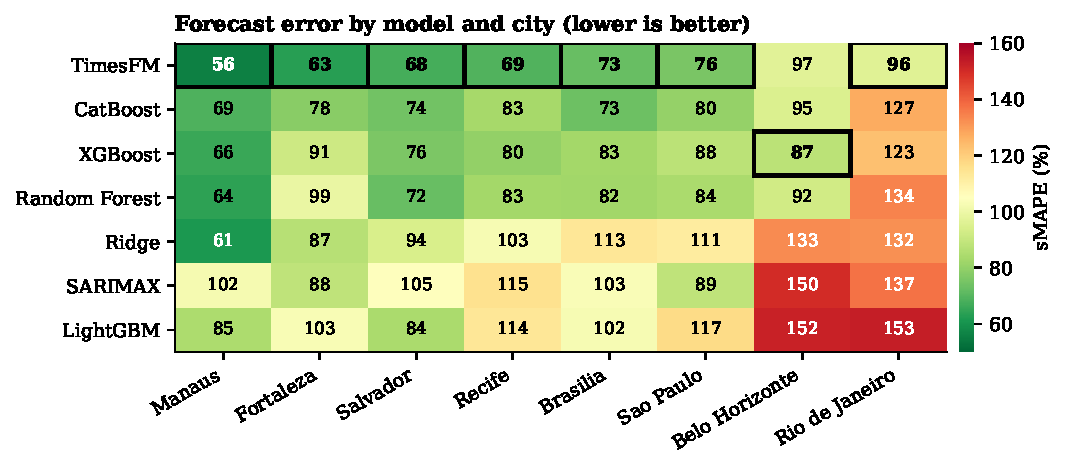
\includegraphics[width=\textwidth]{fig2_heatmap.pdf}
\caption{sMAPE by model and city. Cities are ordered by the lowest error achieved by any
model and models by mean sMAPE across cities. The outlined cell in each column is the
best model for that city. TimesFM holds the best cell in seven of eight columns; Belo
Horizonte is the exception.}
\label{fig:heatmap}
\end{figure}

\begin{figure}[htbp]
\centering
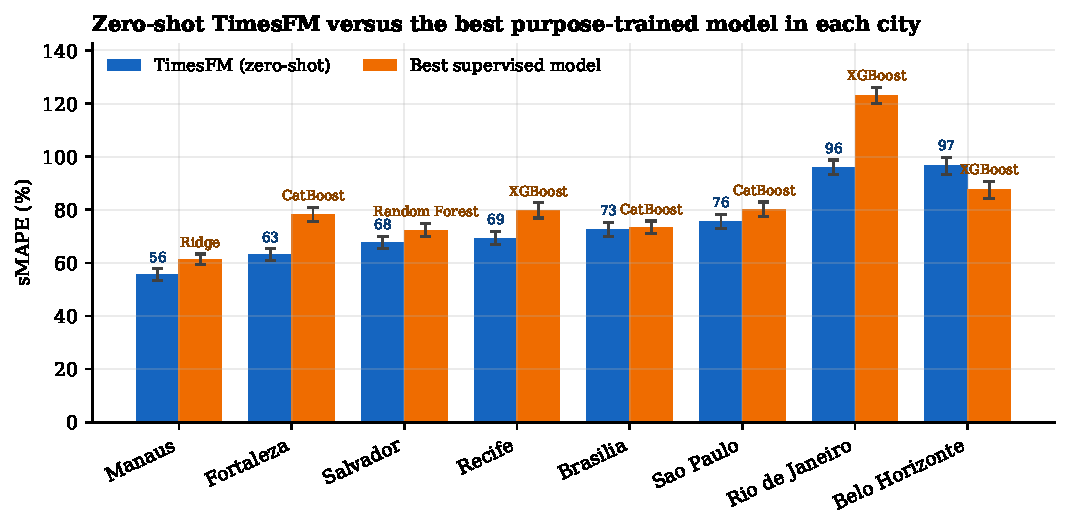
\includegraphics[width=\textwidth]{fig3_timesfm_vs_best.pdf}
\caption{Zero-shot TimesFM against the best purpose-trained model in each city, with 95\%
bootstrap intervals. The label above each orange bar names which supervised model
achieved it, which differs by city. Note that the supervised winner is not stable across
cities, whereas TimesFM is a single unmodified model throughout.}
\label{fig:vsbest}
\end{figure}

\subsection{Absolute error}

Table~\ref{tab:mae-rmse} reports MAE and RMSE on the case-count scale. By MAE, TimesFM
ranked first in all eight cities, including Belo Horizonte, where it led on sMAPE in
none. The RMSE ranking is less consistent: TimesFM led in four cities, while LightGBM led
in S\~ao Paulo, SARIMAX in Bras\'ilia, Random Forest in Manaus and Ridge in Belo
Horizonte, despite all four ranking poorly on both other metrics in those same cities.
Two of these are near-ties that rounding conceals: Manaus (Random Forest 505.8 against
XGBoost 505.9 cases) and Belo Horizonte, where Ridge leads TimesFM by 190 cases on an
RMSE above 17{,}000 while trailing it by 36 percentage points on sMAPE.

The gap between MAE and RMSE within a city quantifies how much of the total error sits in
a few months. In S\~ao Paulo the best MAE is 9{,}617 cases against an RMSE above 43{,}000
for every model, a ratio consistent with error concentrated almost entirely in epidemic
peaks rather than spread across the series.

% gerado por scripts/build_paper_assets.py -- nao editar a mao
\begin{table}[htbp]
\centering
\small
\setlength{\tabcolsep}{4pt}
\caption{Forecasting accuracy by model and city: mean absolute error (MAE) and root
mean squared error (RMSE), in notified cases per month.}
\label{tab:mae-rmse}
\begin{tabular}{llccccccc}
\toprule
City & Metric & TimesFM & CatBoost & XGBoost & Random Forest & SARIMAX & Ridge & LightGBM \\
\midrule
\multirow{2}{*}{Sao Paulo} & MAE & \textbf{8,759} & 9,142 & 10,074 & 9,659 & 76,493 & 11,300 & 10,283 \\
 & RMSE & 41,532 & 41,327 & 41,603 & 41,331 & 1,314,044 & 43,506 & \textbf{40,821} \\[2pt]
\multirow{2}{*}{Rio de Janeiro} & MAE & \textbf{1,899} & 4,487 & 8,357 & 7,368 & 2,481 & 4,920 & 5,507 \\
 & RMSE & \textbf{5,801} & 8,039 & 17,102 & 13,349 & 6,081 & 8,427 & 8,071 \\[2pt]
\multirow{2}{*}{Belo Horizonte} & MAE & \textbf{6,177} & 7,997 & 8,715 & 8,860 & 11,198 & 8,060 & 14,877 \\
 & RMSE & 16,840 & 17,631 & 20,454 & 18,749 & 21,838 & \textbf{16,684} & 21,097 \\[2pt]
\multirow{2}{*}{Brasilia} & MAE & 3,686 & \textbf{3,668} & 4,142 & 4,049 & 4,250 & 4,118 & 4,395 \\
 & RMSE & 12,444 & 11,989 & 12,456 & 12,155 & 12,032 & 12,315 & \textbf{11,678} \\[2pt]
\multirow{2}{*}{Fortaleza} & MAE & \textbf{1,417} & 1,960 & 3,291 & 3,386 & 1,856 & 1,935 & 3,053 \\
 & RMSE & \textbf{2,602} & 3,032 & 5,276 & 4,568 & 3,102 & 2,882 & 3,971 \\[2pt]
\multirow{2}{*}{Recife} & MAE & \textbf{755} & 1,159 & 1,160 & 1,173 & 1,345 & 1,159 & 1,700 \\
 & RMSE & \textbf{1,428} & 1,824 & 1,942 & 1,866 & 2,327 & 1,994 & 2,218 \\[2pt]
\multirow{2}{*}{Manaus} & MAE & \textbf{274} & 343 & 359 & 305 & 352 & 274 & 429 \\
 & RMSE & 556 & 578 & 634 & 531 & 618 & \textbf{529} & 641 \\[2pt]
\multirow{2}{*}{Salvador} & MAE & \textbf{416} & 472 & 517 & 502 & 595 & 518 & 567 \\
 & RMSE & \textbf{687} & 726 & 781 & 742 & 917 & 758 & 765 \\[2pt]
\bottomrule
\end{tabular}

\vspace{0.5em}
\begin{minipage}{\textwidth}
\footnotesize
Bold indicates the best value in each row. MAE and RMSE are reported on the original
case-count scale and are therefore not comparable across cities. RMSE penalises large
errors more heavily than MAE; the gap between the two within a city reflects how much
of the total error is concentrated in a small number of epidemic peaks.
\end{minipage}
\end{table}


\subsection{The metrics disagree}
\label{sec:disagreement}

Table~\ref{tab:metric-disagreement} and Figure~\ref{fig:disagreement} make explicit a
result that a single-metric report would hide: sMAPE, MAE and RMSE select the same model
in only four of the eight cities. Belo Horizonte is the extreme case: each of the three
metrics names a different winner. XGBoost wins on sMAPE, and the headline claim of this
study fails there; TimesFM wins on MAE; Ridge, which has the worst sMAPE of any model in
that city at 133.0\%, wins on RMSE. All three statements are true, and which one is
reported determines whether Belo Horizonte reads as a counterexample.

The mechanism is arithmetic rather than epidemiological. sMAPE normalises each error by
the magnitude of the observation, so the many low-count months between epidemics dominate
it. RMSE squares the error, so the few epidemic months dominate instead. A model that
tracks the baseline well and misses peaks scores well on sMAPE and badly on RMSE, and the
reverse also holds. We therefore report the primary metric as declared in advance and
present the other two alongside rather than selecting the metric that favours a
conclusion.

% gerado por scripts/build_paper_assets.py -- nao editar a mao
\begin{table}[htbp]
\centering
\small
\caption{Best-performing model per city under each accuracy metric, showing where the
choice of metric changes the winner.}
\label{tab:metric-disagreement}
\begin{tabular}{llllc}
\toprule
City & Best by sMAPE & Best by MAE & Best by RMSE & All three agree \\
\midrule
Sao Paulo & TimesFM & TimesFM & LightGBM & No \\
Rio de Janeiro & TimesFM & TimesFM & TimesFM & Yes \\
Belo Horizonte & XGBoost & TimesFM & Ridge & No \\
Brasilia & TimesFM & TimesFM & SARIMAX & No \\
Fortaleza & TimesFM & TimesFM & TimesFM & Yes \\
Recife & TimesFM & TimesFM & TimesFM & Yes \\
Manaus & TimesFM & TimesFM & Random Forest & No \\
Salvador & TimesFM & TimesFM & TimesFM & Yes \\
\bottomrule
\end{tabular}

\vspace{0.5em}
\begin{minipage}{\textwidth}
\footnotesize
The three metrics select the same model in 4 of the eight cities. sMAPE weights
relative error and therefore rewards accuracy during inter-epidemic troughs, when case
counts are low; RMSE weights absolute squared error and therefore rewards accuracy at
epidemic peaks. Reporting a single metric would conceal this disagreement, so the
primary metric is declared in advance (sMAPE) and the others are reported alongside it.
\end{minipage}
\end{table}


\begin{figure}[htbp]
\centering
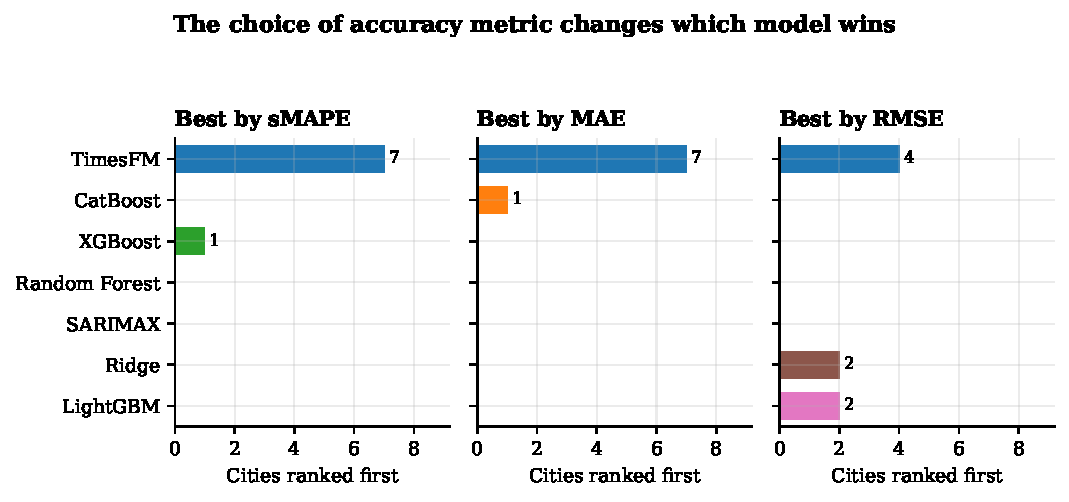
\includegraphics[width=\textwidth]{fig4_metric_disagreement.pdf}
\caption{Number of cities in which each model ranks first, under each of the three
accuracy metrics. The ranking is stable under sMAPE and MAE and fragments under RMSE,
where models that perform poorly overall win individual cities by being conservative at
epidemic peaks.}
\label{fig:disagreement}
\end{figure}

\subsection{No model anticipated the 2024 epidemic}

Figure~\ref{fig:obspred} plots observed against predicted counts for four representative
cities. The 2024 epidemic, the largest in Brazilian records
\citep{GurgelGoncalves2024}, is missed by both the best zero-shot and the best supervised
model in every panel. In S\~ao Paulo the observed peak exceeds 330{,}000 monthly cases
while both model traces remain near baseline. This is the practical ceiling on all
results reported above: the ranking describes which model is least wrong across ordinary
months, not which model would have warned a health authority in 2024.

\begin{figure}[htbp]
\centering
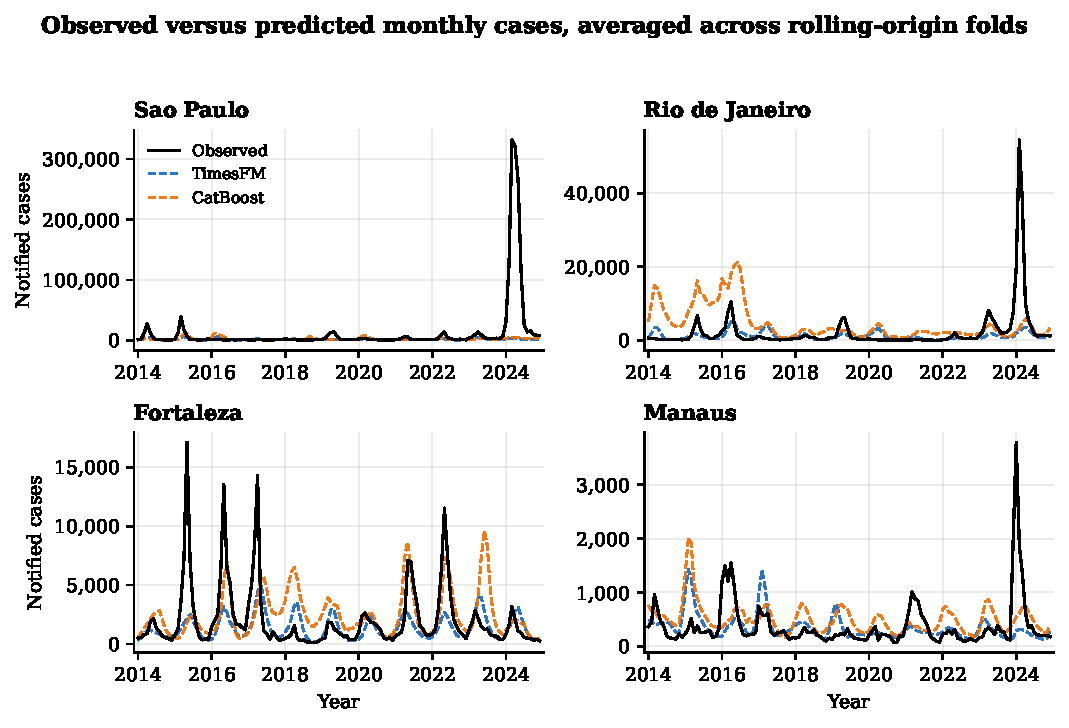
\includegraphics[width=\textwidth]{fig5_observed_vs_predicted.pdf}
\caption{Observed and predicted monthly cases in four cities, with predictions averaged
across all rolling-origin folds covering each month. Both models track the inter-epidemic
baseline and neither reproduces the 2024 peak. CatBoost is shown as the best
purpose-trained model by mean sMAPE.}
\label{fig:obspred}
\end{figure}

\subsection{Temporal and space-time clusters}
\label{sec:clusters}

\missing{Entire subsection. Requires the SaTScan analysis described in Methods: high-rate
purely temporal clusters per city, the space-time scan across all eight cities, and
low-rate clusters marking inter-epidemic troughs, each with start and end dates, observed
and expected counts, relative risk, log likelihood ratio and $p$-value. Nothing in this
subsection can be written from the data currently in the repository.}

% =============================================================================
\section{Discussion}

\subsection{Main findings}

Across eight Brazilian state capitals and 15 years of surveillance data, a foundation
model applied with no local training matched or exceeded six purpose-trained models at a
12-month horizon. It ranked first by sMAPE in seven of eight cities and by MAE in all
eight. The comparison is asymmetric in TimesFM's disfavour: the supervised models were
refitted on each city at each of 121 folds, while TimesFM saw the series only as context
at inference.

The operational consequence is about cost rather than accuracy. The best supervised model
is not the same model in every city: four different ones take that place across the eight
capitals, CatBoost in three, XGBoost in three, Random Forest in Recife and Ridge in
Manaus (Figure~\ref{fig:vsbest}). A per-city pipeline therefore requires per-city model
selection, retraining and monitoring, and the selection itself consumes data that could
otherwise be used for fitting. A single unmodified foundation model removes that
overhead, which is what makes extension to municipalities without modelling capacity
plausible.

That said, the accuracy in absolute terms is poor everywhere. A mean sMAPE of 75\% is not
a small error, and no model anticipated the 2024 epidemic in any city. The honest
reading is that these models provide a reasonable baseline expectation for planning under
ordinary conditions and are not outbreak detectors.

\subsection{Comparison with the literature}

Published Brazilian benchmarks have largely compared ARIMA variants against tree ensembles
over short horizons and often a single city
\citep{Roster2022,Chen2025rj,Sebastianelli2024}. Their consistent finding, that
tree-based models beat classical parametric ones on volatile dengue series
\citep{Fang2024}, is reproduced here: every tree ensemble except LightGBM outperformed
SARIMAX on the primary metric. Our contribution is to show that the additional step from
purpose-trained ensembles to a zero-shot foundation model is achievable without
sacrificing accuracy. The magnitude of the gain over SARIMAX, roughly 30 sMAPE points on
average, is of the same order as the gains that dynamic ensemble approaches have reported
against fixed parametric models on Brazilian dengue data \citep{McGough2021}.

Neural approaches to dengue forecasting, including LSTM architectures applied across
Brazil, need substantial per-city history and degrade under distribution shift
\citep{Chen2025lstm}. Zero-shot inference sidesteps both problems by construction,
though it introduces a different dependency: performance rests on how well the
pre-training corpus covers epidemic-like dynamics, which is not inspectable.

The 12-month horizon here is considerably longer than the 4 to 8 weeks typical of
published dengue benchmarks. That makes these results relevant to annual planning cycles
and correspondingly less relevant to short-term outbreak response, and it also makes the
error magnitudes not directly comparable to the short-horizon literature.

\subsection{Belo Horizonte}

Belo Horizonte is the one city where a supervised model leads on the primary metric, and
it is worth being precise about what that means. XGBoost leads on sMAPE, TimesFM on MAE,
and Ridge on RMSE. The city's series combines sharp high-magnitude peaks with long near-zero
troughs, a profile that lag features capture well and that penalises a model normalising
error by observation magnitude. Cities with this signature are candidates for a hybrid
arrangement in which foundation model output is corrected by a locally fitted residual
model, but that design was not tested here and we make no claim about its performance.

\subsection{Limitations}

Seven limitations bound these conclusions.

First, the outcome is notified cases, which under-represent true infections
\citep{Siqueira2022}. What is forecast is the behaviour of the surveillance system,
including reporting delay and saturation during peaks, not biological incidence.

Second, no exogenous covariates were used. Models with access to rainfall, temperature
and vector indices outperform univariate approaches for outbreak onset
\citep{Barcellos2024,Fang2024}, so the TimesFM advantage may narrow or reverse once
supervised models receive informative features that a zero-shot model cannot consume.

Third, no probabilistic forecasts were produced and therefore no calibration was
assessed. TRIPOD+AI requires calibration to be reported, and for point forecasts of this
kind it cannot be. Without prediction intervals, a health authority cannot know how much
confidence to place in any single forecast. This is the most consequential gap in the
present analysis and the first thing a subsequent version should add.

Fourth, the bootstrap intervals resample predictions that are serially dependent within
and across folds. They understate uncertainty and are reported as a lower bound, not as a
significance test. Where intervals overlap, as in S\~ao Paulo, no advantage is claimed.

Fifth, validation is internal and temporal. No independent surveillance system,
country or held-out cohort was used, and the eight cities constitute eight internal
validations rather than a geographic external validation.

Sixth, SARIMAX orders and all tree hyperparameters were fixed rather than tuned. This
mirrors low-maintenance deployment but understates what a carefully tuned supervised
pipeline could achieve, which makes the comparison conservative in TimesFM's favour on
maintenance cost and potentially generous on accuracy.

Seventh, one TimesFM checkpoint was evaluated on eight capitals. Whether the result holds
for other foundation models \citep{Ansari2024chronos,Woo2024moirai}, other checkpoints,
or the smaller municipalities with shorter and more irregular reporting histories that
make up most of Brazil, is untested.

\subsection{Conclusion}

A zero-shot foundation model matched or exceeded six purpose-trained models for
12-month-ahead dengue forecasting in eight Brazilian state capitals, without any
city-specific training, and did so under a validation design that gave its competitors
repeated access to local data it never saw. This supports evaluating foundation models as
a low-maintenance forecasting layer within InfoDengue, particularly for municipalities
where maintaining a bespoke model is not feasible. It does not support using these
forecasts as outbreak triggers: absolute error remained high in every city, and no model
anticipated the 2024 epidemic. Adding prediction intervals and assessing calibration are
prerequisites for operational use.

% =============================================================================
\section*{Declarations}

\paragraph{Ethics approval.} Not required. The study used publicly available aggregate
surveillance data containing no individual-level records.

\paragraph{Data and code availability.} Monthly case data are publicly available through
the InfoDengue API (\url{https://info.dengue.mat.br/api/}). All analysis code, processed
data, result files and the scripts that generate every table and figure in this
manuscript are available at \url{https://github.com/fabianofilho/dengue-time-series}.

\paragraph{Funding.} No external funding was received.

\paragraph{Conflicts of interest.} The authors declare no conflicts of interest.

\paragraph{Author contributions.} \missing{CRediT contribution statement for each of the
three authors.}

\paragraph{Use of artificial intelligence.} The authors used a large language model based
assistant to support literature organisation, drafting and the generation of analysis and
figure code. The tool is not an author. The authors reviewed and verified all content,
including every reported number against the underlying analysis output, and take full
responsibility for the integrity and accuracy of the work.

\paragraph{Acknowledgements.} Surveillance data were obtained from InfoDengue
(Fiocruz/FGV). TimesFM was developed by Google DeepMind and distributed through
HuggingFace.

% =============================================================================
\bibliographystyle{plainnat}
\bibliography{refs/references}

\end{document}
